%%%%%%%%%%%%%%%%%%%%%%%%%%%%%%%%%%%%%%%%%
% Short Sectioned Assignment LaTeX Template Version 1.0 (5/5/12)
% This template has been downloaded from: http://www.LaTeXTemplates.com
% Original author:  Frits Wenneker (http://www.howtotex.com)
% License: CC BY-NC-SA 3.0 (http://creativecommons.org/licenses/by-nc-sa/3.0/)
%%%%%%%%%%%%%%%%%%%%%%%%%%%%%%%%%%%%%%%%%

%----------------------------------------------------------------------------------------
%   PACKAGES AND OTHER DOCUMENT CONFIGURATIONS
%----------------------------------------------------------------------------------------

\documentclass[10pt,a4paper,spanish]{article}

% ---- Entrada y salida de texto -----

\usepackage[spanish]{babel} 
\usepackage[T1]{fontenc} % Use 8-bit encoding that has 256 glyphs
\usepackage[utf8]{inputenc}
\usepackage{cite}
% \usepackage{spreadtab}
% \usepackage{fourier} % Use the Adobe Utopia font for the document - comment this line to return to the LaTeX default
\usepackage[usenames, dvipsnames]{color}
\usepackage[table]{xcolor}
\usepackage{colortbl}
\usepackage[bookmarks=true,colorlinks=true,linkcolor=red,citecolor=blue]{hyperref}
% \usepackage{cite}
% \usepackage[official]{eurosym}
\usepackage{tikz}
% \usepackage{pgfplots}
% \pgfplotsset{compat=1.5}

\usepackage{subfigure}

% \usepackage{pseudocode}

% ---- Otros paquetes ----
\usepackage{enumerate}
\usepackage{amsmath,amsfonts,amsthm,amssymb} % Math packages
\usepackage{graphics,graphicx} %para incluir imágenes y notas en las imágenes
% Para hacer tablas comlejas
%\usepackage{multirow}
%\usepackage{threeparttable}

\usepackage[a4paper, margin=1.3in]{geometry}


\usepackage{sectsty} % Allows customizing section commands
\allsectionsfont{\centering \normalfont\bfseries\scshape} % Make all sections centered, the default font and small caps
\usepackage{fancyhdr}
\pagestyle{fancy}
%con esto nos aseguramos de que las cabeceras de capítulo y de sección vayan en minúsculas

\renewcommand{\sectionmark}[1]{%
      \markright{\thesection\ #1}}
\fancyhf{} %borra cabecera y pie actuales
\fancyhead[LE,RO]{{\bfseries Práctica 4}}
\fancyhead[LO]{\bfseries Marta Gómez}
\fancyfoot[C]{\thepage{}}
\renewcommand{\headrulewidth}{0.5pt}
\renewcommand{\footrulewidth}{0pt}
\addtolength{\headheight}{0.5pt} %espacio para la raya
\fancypagestyle{plain}{%
      \fancyhead{} %elimina cabeceras en páginas "plain"
      \renewcommand{\headrulewidth}{0pt} %así como la raya
}

\numberwithin{equation}{section} % Number equations within sections (i.e. 1.1, 1.2, 2.1, 2.2 instead of 1, 2, 3, 4)
\numberwithin{figure}{section} % Number figures within sections (i.e. 1.1, 1.2, 2.1, 2.2 instead of 1, 2, 3, 4)
\numberwithin{table}{section} % Number tables within sections (i.e. 1.1, 1.2, 2.1, 2.2 instead of 1, 2, 3, 4)

\setlength\parindent{0pt} % Removes all indentation from paragraphs - comment this line for an assignment with lots of text
\setlength{\parskip}{1ex plus 0.5ex minus 0.2ex}

\newcommand{\horrule}[1]{\rule{\linewidth}{#1}} % Create horizontal rule command with 1 argument of height

%----------------------------------------------------------------------------------------
%   TÍTULO Y DATOS DEL ALUMNO
%----------------------------------------------------------------------------------------

\title{
\normalfont \normalsize 
{\bf Redes y Sistemas Complejos} \\ Curso 2016-2017 \\ [25pt] % Your university, school and/or department name(s)
\horrule{0.5pt} \\[0.4cm] % Thin top horizontal rule
\huge \textsc{Práctica 4: \\ Estudio Comparativo de Métodos \\ para Poda y Visualización \\ de Redes } \\ % The assignment title
\horrule{2pt} \\[0.5cm] % Thick bottom horizontal rule
}

\author{\textit{Marta Gómez Macías}} %\\ \texttt{mgmacias95@correo.ugr.es} \\ 75929776Z \\[0.5cm]

% \date{\normalsize\today} % Incluye la fecha actual

% \usepackage{pdflscape}

%----------------------------------------------------------------------------------------
% DOCUMENTO
%----------------------------------------------------------------------------------------

\begin{document}
%Cambiar Cuadros por Tablas y lista de...
\renewcommand{\listtablename}{Índice de tablas}
\renewcommand{\tablename}{Tabla} 

\begin{titlepage}
\begin{center}

\includegraphics[width=0.2\textwidth]{../../ugr}

\normalfont \normalsize 
{\bf Redes y Sistemas Complejos} \\ Curso 2016-2017 \\ [25pt] % Your university, school and/or department name(s)
\horrule{0.5pt} \\[0.4cm] % Thin top horizontal rule
{\huge \textsc{Práctica 4: \\ Caso Práctico de Análisis \\ y Evaluación de \\ Redes}} % The assignment title
\horrule{2pt} \\[0.5cm] % Thick bottom horizontal rule

{\Large \textit{Marta Gómez Macías} \\ \texttt{mgmacias95@correo.ugr.es} \\ 75929776Z \\[0.5cm]

\date{\today}} % Incluye la fecha actual
\end{center}
\end{titlepage}

\tableofcontents % para generar el índice de contenidos

% \listoffigures

% \listoftables

\section{Selección del dominio, definición de la pregunta y obtención del conjunto estructural inicial}

\subsection{Selección del dominio y definición de la pregunta}
Llevo muchos años participando activamente en la red social \textit{Twitter}. Durante estos años, he ido siguiendo (y dejando de seguir también) a un montón de gente muy diferente: amigos del instituto, cuentas que ponen tweets interesantes, amigos de la facultad, etc. En mi \textit{Timeline} veo tweets de todo tipo y muy diferentes entre sí, tanto que a veces se me hace algo confuso. Por tanto, me hice la siguiente pregunta: \textbf{¿podría agrupar de una forma sencilla todas las cuentas que sigo por su temática?}

Dándole vueltas a esta pregunta, apliqué la siguiente lógica: los amigos de la facultad que sigo en Twitter, también se siguen entre sí. Al igual que los del instituto o la gente que conocí en un determinado evento. Es decir, si dos de las cuentas que sigo se siguen entre sí, es bastante probable que publiquen Tweets sobre temas muy similares. Así, descubrí que viendo las comunidades que hay entre mis ``amigos'' de Twitter podría agrupar las diferentes cuentas que sigo por temática.

\subsection{Obtención del conjunto estructural inicial}
Para obtener los datos, he desarrollado una sencilla aplicación con \textit{Django} y \textit{Tweepy}. He creado una base de datos en \texttt{sqlite3} en la que voy guardando usuarios de Twitter y las personas a las que siguen. Dicha aplicación se encuentra libre en \href{https://github.com/mgmacias95/TwitterFriends}{Github}.

La aplicación, en primer lugar, almacena en la base de datos todas las personas que sigo y, además, todos los usuarios que siguen las personas a las que sigo. Una vez tengo registrados todos mis amigos y los amigos de mis amigos, los relaciono entre sí usando los \texttt{ManyToManyField} de \textit{Django}. Es importante destacar que esta red es \textit{dirigida}, ya que en Twitter un usuario no tiene por qué hacer \textit{follow back}.

Finalmente, como sólo me interesa quedarme con las relaciones entre las personas que yo sigo, hago un filtrado a la hora de exportar la red a formato GDF. Si no hubiese hecho ningún filtrado, trabajaría con una red de 100.000 nodos, que fue los que recopilé en primer lugar.

\section{Construcción de la red compleja a analizar y visualizar}
En mi caso, la red obtenida era bastante pequeña, ya que sólo sigo a unas 540 personas. Por tanto, no he eliminado ningún nodo. Tampoco he eliminado ningún enlace, ya que todos los enlaces tienen el mismo peso y, si elimino algún enlace, pierdo la relación entre dos usuarios. 

Por tanto, debido a la naturaleza de mi red, no me ha sido necesario aplicar una poda Pathfinder o algún filtro.

El único nodo que he eliminado ha sido el nodo correspondiente a mi usuario de Twitter.

\section{Cálculo de los valores de las medidas de análisis}

\begin{table}[!h]
\centering
\begin{tabular}{cc}
\textbf{Medida} & \textbf{Valor} \\
\hline
$N$ & $542$ \\
$L$ & $6470$ \\
$D$ & $0.022$ \\
$<k>$ & $23.875$ \\
$d_{max}$ & $11$ \\
$<d>$ & $3.500166852057842$ \\
$<d_{aleatoria}>$ & $1.7255717255717256$ \\
$<C>$ & $0.264$ \\
$<C_{aleatoria}>$ & $1.726$ \\
Número de componentes conexas & $60$ \\
$N_{componente\;gigante}$ & $482$ ($88.93\%$) \\
$L_{componente\;gigante}$ & $6468$ ($99.97\%$) \\
\end{tabular}
\caption{Valores de las medidas globales básicas}
\label{basicglobal}
\end{table}

\begin{figure}[!h]
    \centering
    \mbox{
        \subfigure[Distribución del grado de entrada]{
            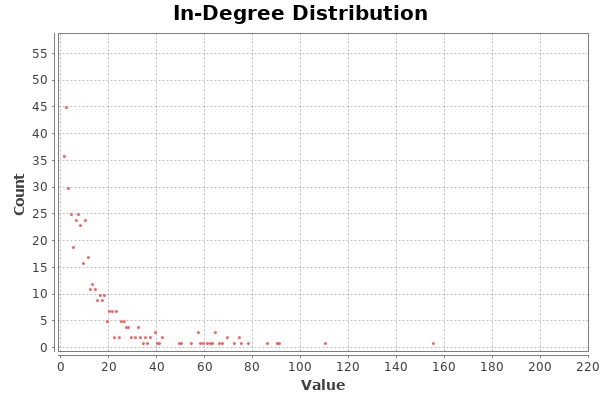
\includegraphics[width=0.5\textwidth]{degree-report/indegree-distribution}
            \label{din}
        }
        \subfigure[Distribución del grado de salida]{
            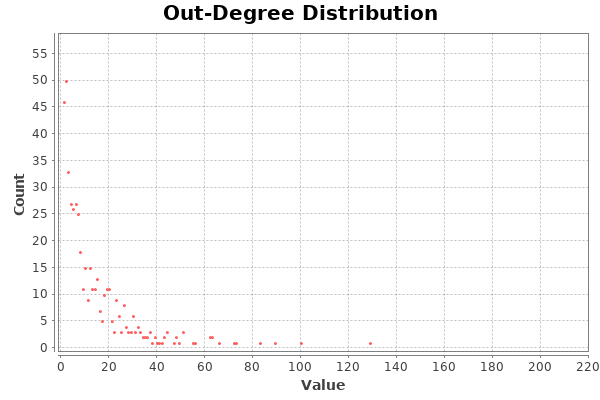
\includegraphics[width=0.5\textwidth]{degree-report/outdegree-distribution}
            \label{dout}
        }
    }
    \caption{Gráficos de distribución del grado de entrada y salida}
    \label{degree}
\end{figure}

\begin{figure}[!h]
    \centering
    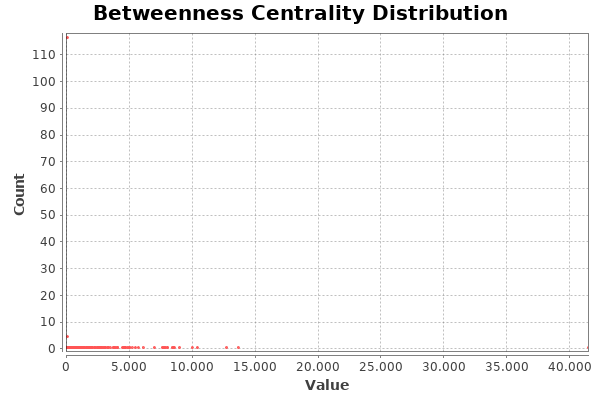
\includegraphics[width=0.5\textwidth]{distance-report/Betweenness-Centrality-Distribution}
    \caption{Gráfico de distribución de la intermediación}
    \label{bet}
\end{figure}

\begin{figure}[!h]
    \centering
    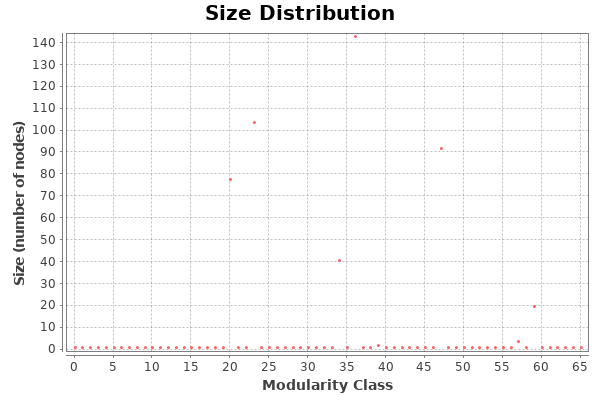
\includegraphics[width=0.5\textwidth]{modularity-report/communities-size-distribution}
    \caption{Gráfico de distribución de las 66 distintas comunidades en la red}
    \label{com}
\end{figure}

\end{document}

